\chapter{Características-chaves em aplicações SGX}
\label{chapter:abordagem}

Neste capítulo, detalhamos a abordagem utilizada neste trabalho, que envolve a
avaliação do impacto de características de aplicações SGX na performance e na
segurança providas pelas mesmas. Para cada uma das características avaliadas
neste trabalho, realizamos vários experimentos. Para os experimentos dispomos de
uma máquina Dell Optiplex 5040, com um processador Intel Core i7-7700, com 4
núcleos operando a $3,4\ GHz$, e $8\ GB$ de memória principal disponível.

De forma a mensurar o impacto de cada uma das características, coletamos e
analisamos duas métricas: ($i$) o tamanho do TCB gerado -- lembrando que quanto
maior o TCB, maior a probabilidade de se inserir \textit{bugs} e
vulnerabilidades no mesmo -- impactando diretamente a segurança de uma
aplicação, e ($ii$) tempo de processamento das aplicações.

Em cada uma das seções a seguir, apresentamos as principais características que
devem ser consideradas durante o desenvolvimento de aplicações SGX, incluindo
uma descrição dos experimentos realizados, resultados obtidos nos experimentos,
e uma discussão sobre os impactos de tais características nas aplicações em
questão.  

\section{Gerência de memória}
\label{sec:abordagem_gerencia_memoria}

Conforme apontado na Seção~\ref{sec:sgx_limitacoes}, uma das limitações de SGX é
a pequena área de memória protegida pela tecnologia, com apenas $128\ MB$
disponíveis.
Nesta seção, avaliamos os possíveis impactos na performance de aplicações SGX,
caso elas venham a ter um consumo de memória que exceda o limite de memória
disponível.

\begin{lstlisting}[language=C, label=lst:acesso_aleatorio, caption={Pseudocódigo
do experimento de acesso aleatório à memória.}]
    #define MB_SIZE 1024*1024

    char tmp;

    char perform_random_memory_access(int size_in_mb) {
        size_t total_size = size_in_mb * MB_SIZE;
        char *allocated_memory = (char *) malloc(total_size);
        
        int i;
        for (i=0; i<total_size; ++i) {
            int pos = rand() % total_size; // A função rand() gera um número aleatório.
            tmp ^= allocated_memory[pos]; // Para evitar otimizações feitas pelo compilador.
        }
        free(allocated_memory);
        return tmp;
    }
\end{lstlisting}

\subsection*{Experimentos}

Para avaliar o impacto do consumo de memória em aplicações SGX, realizamos um
experimento que compara o desempenho de acesso aleatório à memória em uma
aplicação escrita em C, sem garantias de segurança, e em uma aplicação que usa
SGX, com garantias de segurança. As implementações de ambas aplicações são
praticamente idênticas, diferindo apenas que a alocação e acesso aleatório de
memória da aplicação SGX são feitos dentro de um enclave, enquanto na primeira
implementação são feitos de forma insegura.

O código utilizado em ambas implementações é exibido no Código Fonte~\ref
{lst:acesso_aleatorio}, e é descrito da seguinte forma:

\begin{enumerate}
    \item A aplicação aloca um espaço de memória do tamanho passado como
    parâmetro, associando-o à variável \textit{allocated\_memory}, que será
    utilizada como um \textit{array} de elementos do tipo \textit{char}
    (linha 7);
    \item A aplicação gera um número inteiro aleatório $pos$, que indica o
    índice do \textit{array} a ser acessado (linha 11);
    \item A aplicação acessa o elemento presente no índice aleatório gerado
    (linha 12);
    \item A aplicação repete os passos 2 e 3 pelo número de vezes que
    corresponde ao total de posições do \textit{array} alocado (linhas 10-13);
    \item A aplicação libera o espaço alocado para a variável \textit
    {allocated\_memory} (linha 14).
\end{enumerate}

Neste experimento o espaço de memória utilizado pelas aplicações foi variado
entre $1\ MB$ e $1024\ MB$, em uma escala logarítmica.

Tendo em vista que, neste experimento, apenas o tamanho da memória alocada e
acessada aleatoriamente é variada, coletamos apenas a métrica do tempo de
processamento tanto para a aplicação insegura, em C puro, e a aplicação segura,
utilizando SGX.

\subsection*{Resultados obtidos}

\begin{figure*}[!t]
    \centering
    \subfloat[Tamanho de memória variando entre 1MB e 1024MB]
    {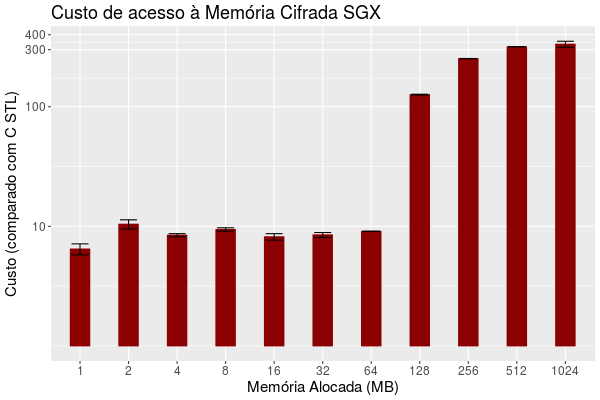
\includegraphics[width=5in]{img/memory-benchmark-1-1024-br}
    \label{fig:sgx_memory_overhead_1024}}
    \hfil
    \subfloat[Tamanho de memória variando entre 64MB e 128MB]
    {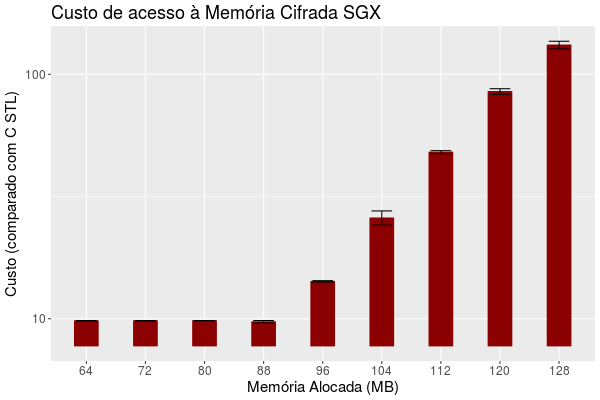
\includegraphics[width=5in]{img/memory-benchmark-64-128-br}
    \label{fig:sgx_memory_overhead_64}}
    \caption{Sobrecarga média de acesso à memória SGX comparado com acesso à
    memória em C puro, com um intervalo de 95\% de confiança.}
    \label{fig:sgx_memory_overhead}
\end{figure*}

Para cada uma das configurações descritas anteriormente, trinta repetições do
experimento foram executadas.
A Figura \ref{fig:sgx_memory_overhead} mostra a relação entre os tempos de
execução da aplicação SGX e da aplicação C pura, considerando cada uma das
configurações determinadas anteriormente. Na Figura~\ref
{fig:sgx_memory_overhead_1024}, notamos que aplicações SGX que usam até $64\ MB$ de
memória têm um custo médio de acesso à memória aproximadamente $10$ vezes mais
alto que aplicações sem garantias de segurança. Já aplicações que consumam $128\ MB$
de memória ou mais têm um custo médio de acesso à memória pelo menos $100$ vezes,
e chegando a ser $380$ vezes mais alto que o de aplicações inseguras.

Para entender melhor o comportamento do custo de acesso à memória em aplicações
SGX, repetimos o experimento descrito anteriormente, porém variando o espaço de
memória utilizado entre $64\ MB$ e $128\ MB$, com incrementos de $8\ MB$. Na Figura~\ref
{fig:sgx_memory_overhead_64}, podemos observar que aplicações que demandam até
88MB de memória têm um custo médio de acesso à memória $10$ vezes mais alto que
aplicações inseguras. Aplicações que ultrapassem $88\ MB$ têm um custo de acesso que
cresce linearmente à medida que mais memória é demandada.

\subsection*{Discussão}

Considerando os resultados obtidos nestes experimentos, podemos concluir que a
quantidade de memória consumida e uma gerência de memória apropriada são
características de extrema importância no desenvolvimento de aplicações SGX,
visto que um alto consumo de memória pode torná-las impraticáveis no mundo real.
Dados os resultados obtidos nos experimentos aqui apresentamos, recomendamos que
desenvolvedores busquem criar e utilizar suas aplicações de um modo que ela não
consuma além do limite de memória disponível na EPC, sob o risco de obter uma
sobrecarga demasiadamente alta no tempo de processamento de sua aplicação, caso
essa recomendação não seja seguida.

É importante notar que, apesar de termos reservado um espaço de $128\ MB$ para a
PRM, apenas cerca de $90\ MB$ ficam disponíveis para a EPC. Isso de deve ao fato de
que parte da PRM é utilizada pela estrutura EPCM e pelos enclaves especiais da
Intel.

\section{Particionamento de dados}
\label{sec:abordagem_particionamento_dados}

Existem aplicações que precisam processar um grande volume de dados, também
conhecido como processamento de \textit{Big Data}. Considerando esse tipo de
aplicações, desejamos analisar qual a melhor forma para processar este grande
volume de dados, desde que sejam independentes entre si. Nesta seção,
procura-se, mais precisamente, saber se, e como, este grande volume de dados
independentes deve ser particionado para ser processado dentro de enclaves SGX,
considerando-se a disponibilidade de um único enclave. Em outras palavras,
deseja-se identificar como particionar um grande volume de dados para processar
suas partes independentes, sequencialmente, da forma mais eficiente possível.

\subsection*{Experimentos}

A característica que avaliamos nesta seção envolve apenas variações na carga
útil a ser processada, e não na aplicação SGX usada para processar estes dados.
Desta forma, o tamanho do TCB não será uma métrica coletada e avaliada nestes
experimentos, uma vez que o tamanho do TCB permanece constante em todas as
configurações. A métrica coletada e avaliada nesta seção é o tempo de execução
necessário para completar a tarefa de computar a soma de todos os elementos de
um \textit{array} de números inteiros com 1GB de tamanho.

Este experimento, foi dividido em duas partes. Em um primeiro momento, buscou-se
avaliar o tempo de processamento do \textit{array}, considerando-se partições
com tamanhos de $1$, $2$, $4$, $8$, $16$, $32$, $64$, $128$, $256$, $512$, e
$1024\ MB$. Em um segundo momento, tendo em vista as observações de perda de
desempenho quando enclaves excedem o tamanho disponível na EPC, feitas na
Seção~\ref{sec:abordagem_gerencia_memoria}, buscou-se avaliar também o tempo de
processamento do \textit{array}, considerando-se partições com tamanhos de $72$,
$80$, $88$, $96$, $104$, e $112\ MB$.

\begin{lstlisting}[language=C, label=lst:particionamento_dados, caption={Pseudocódigo
do experimento de particionamento de dados.}]
    // Na parte insegura da aplicação

    #define MB_SIZE 1024*1024
    
    long sum_array(int chunk_size_in_mb){
        int array_size = 1024 * MB_SIZE;
        int chunk_size = chunk_size_in_mb * MB_SIZE;
        int *array = generate_random_array(array_size); // Cria um array com tamanho 1GB
        long sum = 0;
        int i;
        for (i=0; i<array_size/chunk_size; ++i){
            sum += enclave_sum(&array[i*chunk_size], chunk_size);
        }
        free(allocated_memory);
        return sum;
    }

    // No enclave da aplicação

    long enclave_sum(int *array, int array_size){
        long sum = 0;
        int i;
        for (i=0; i<array_size; ++i){
            sum += array[i];
        }
        return sum;
    }
\end{lstlisting}

O código utilizado neste experimento é exibido no Código Fonte~\ref
{lst:particionamento_dados}, e é descrito da seguinte forma:

\begin{enumerate}
    \item A aplicação aloca um espaço de memória com tamanho de $1\ GB$,
    associando-o à variável \textit{array}, que é um \textit{array} de elementos
    do tipo \textit{int} (linha 8);
    \item A aplicação envia para o enclave uma partição dos dados para calcular
    a soma dos elementos desta partição (linha 12);
    \item O enclave da aplicação calcula a soma dos elementos da partição
    recebida (linhas 23-25);
    \item Repetimos os passos 2 e 3 até que a soma de todas as partições tenham
    sido computadas (linhas 11-13);
    \item A aplicação libera o espaço alocado para a variável \textit{array}
    (linha 14).
\end{enumerate}

É importante salientar que o tamanho do \textit{array} copiado para o enclave a
cada chamada à função \textit{enclave\_sum} é exatamente o tamanho passado pelo
parâmetro \textit{array\_size} da mesma função. O número de chamadas feitas à
função \textit{enclave\_sum}, considerando cada um dos tamanhos de partição
propostos, pode ser visto na Tabela~\ref
{tab:abordagem_particionamento_dados_chamadas}.

\begin{center}
    \begin{table}
        \caption{Número de chamadas à função \textit{enclave\_sum} necessárias
        para computar a soma dos elementos de um \textit{array} com 1GB de
        tamanho, de acordo com o tamanho, em MB, das partições.}
        \label{tab:abordagem_particionamento_dados_chamadas}
        \centering
        \begin{tabular}{|c|c|c|c|c|}
            \cline{1-2} \cline{4-5}
            \textbf{Tam. da partição} & \textbf{Num. de chamadas} & & \textbf{Tam. da partição} & \textbf{Num. de chamadas} \\
            \cline{1-2} \cline{4-5}
            1 & 1024 & & 88 & 12 \\
            \cline{1-2} \cline{4-5}
            2 & 512 & & 96 & 11 \\
            \cline{1-2} \cline{4-5}
            4 & 256 & & 104 & 10 \\
            \cline{1-2} \cline{4-5}
            8 & 128 & & 112 & 10 \\
            \cline{1-2} \cline{4-5}
            16 & 64 & & 120 & 9 \\
            \cline{1-2} \cline{4-5}
            32 & 32 & & 128 & 8 \\
            \cline{1-2} \cline{4-5}
            64 & 16 & & 256 & 4 \\
            \cline{1-2} \cline{4-5}
            72 & 15 & & 512 & 2 \\
            \cline{1-2} \cline{4-5}
            80 & 13 & & 1024 & 1 \\
            \cline{1-2} \cline{4-5}
        \end{tabular}
    \end{table}
\end{center}

\subsection*{Resultados obtidos}

\begin{figure*}[!t]
   \centering
   \subfloat[Tamanho da partição variando entre 1MB e 1024MB]
   {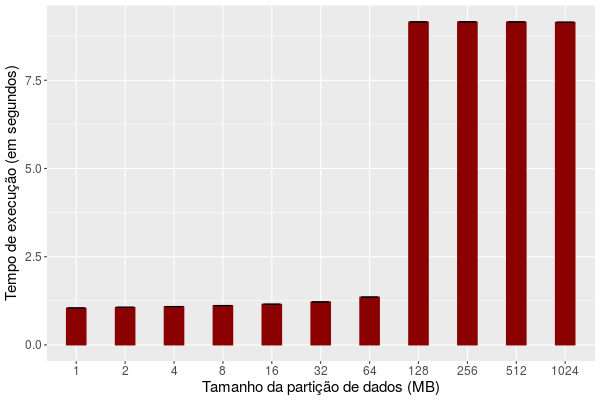
\includegraphics[width=5in]{img/particionamento-dados-1-1024-final}
   \label{fig:abordagem_particionamento_dados_1024}}
   \hfil
   \subfloat[Tamanho da partição variando entre 64MB e 128MB]
   {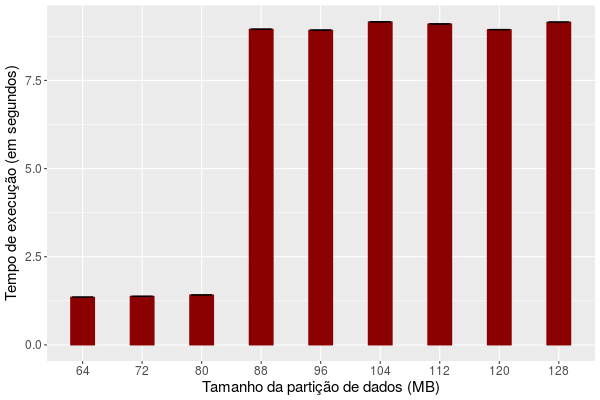
\includegraphics[width=5in]{img/particionamento-dados-64-128-final}
   \label{fig:abordagem_particionamento_dados_128}}
   \caption{Tempos médios para calcular a soma dos elementos de um \textit
   {array} com tamanho de 1GB, variando o tamanho das partições utilizadas
   no cálculo das somas parciais, com um intervalo de 95\% de confiança.}
   \label{fig:abordagem_particionamento_dados}
\end{figure*}

A Figura~\ref{fig:abordagem_particionamento_dados} mostra o tempo total de
processamento do \textit{array} com tamanho de $1\ GB$, em cada um dos cenários
propostos. A partir dos resultados exibidos na Figura~\ref
{fig:abordagem_particionamento_dados_1024}, notamos que, para o particionamento
de dados feito com partições de até $64\ MB$, à medida que o tamanho das partições
cresce, o tempo total de execução da tarefa também cresce -- o tempo de execução
usando partições com tamanho de $64\ MB$ é cerca de $28\%$ mais alto que o tempo de
execução usando partições com tamanho de $1\ MB$. Já para o particionamento de dados
feito com partições de $128\ MB$ ou mais, é notável a sobrecarga gerada pelo consumo
de memória superior ao disponibilizado na EPC, porém não há, estatísticamente,
diferença entre o uso de diferentes tamanhos de partições que excedam este
limite -- o tempo de execução da tarefa usando partições de $1024\ MB$ é cerca de
$0,6\%$ mais baixo que o tempo de execução usando partições de $128\ MB$.

Analisando os dados exibidos na Figura~\ref
{fig:abordagem_particionamento_dados_128}, podemos dizer que a sobrecarga no
tempo de execução da tarefa pode ser observado quando particionamos os dados em
partições com tamanho de $88\ MB$ ou mais, gerando um tempo de execução pelo menos
$534\%$ mais alto que o uso de partições que não extrapolam o limite da EPC.

\subsection*{Discussão}

Mais uma vez, podemos notar que o limite de memória disponível na EPC é um dos
fatores-chave no desenvolvimento de aplicações SGX. Mais especificamente,
mostramos com estes experimentos que é essencial que grandes volumes de dados
sejam particionados antes de serem processados em aplicações SGX. Dados os
resultados obtidos, recomendamos que grandes volumes de dados sejam
particionados em pedaços tão pequenos quanto possível, e evitar a todo custo
processar pedaços de dados que excedam o tamanho de $80\ MB$.

\section{Particionamento de aplicações}
\label{sec:abordagem_particionamento_aplicacoes}

Conforme exposto na Seção~\ref{sec:sgx_modelo_programacao}, aplicações SGX são
divididas entre parte segura, \textit{i.e.}, enclave que protege dados contra
modificação ou acesso não autorizados, e parte insegura, \textit{i.e.}, código
em volta do enclave, que serve para processar dados não-sensíveis, e  para
estabelecer uma comunicação entre o enclave e outras aplicações. Desta forma,
nesta seção, buscamos analisar qual a melhor forma de particionar aplicações
SGX, de modo que sua performance e sua segurança não sejam comprometidas.

\subsection*{Experimentos}

A característica que avaliamos nesta seção envolve variações na divisão de uma
aplicação, com o objetivo de torná-la segura, através do uso de SGX. Deste modo,
coletamos tanto o tempo de execução necessário para completar a tarefa de
computar a soma de um número variado de elementos, como fazemos considerações
sobre o TCB resultante.

Neste experimento, consideramos uma aplicação simples, que tem como funções
($i$) gerar e ($ii$) computar a soma de uma quantidade $N$ de números inteiros.
Para realizar esta tarefa, consideramos duas implementações. A primeira delas,
exibida no Código Fonte~\ref{lst:particionamento_aplicacoes_enclave}, realiza
ambas as funções dentro do enclave, gerando um maior TCB, mas mantendo todo o
processamento dentro do enclave, e é descrita da seguinte forma:

\begin{enumerate}
    \item O enclave inicializa a variável \textit{sum} com o valor $0$ (linha
    10);
    \item O enclave gera um novo número (linhas 3-7 e linha 13);
    \item O enclave soma o novo número à variável \textit{sum} (linha 14);
    \item O enclave repete $N$ vezes os passos 2 e 3, até obter o resultado
    final (linhas 12-15).
\end{enumerate}


A segunda implementação, exibida no Código Fonte~\ref
{lst:particionamento_aplicacoes_mista}, por sua vez, realiza a função de somar
os elementos dentro do enclave, enquanto a função de gerar o próximo elemento é
realizada pela parte insegura da aplicação, gerando um TCB reduzido, mas
executando um grande número interações entre as partes segura e insegura através
de OCalls. Esta implementação é descrita da seguinte forma:

\begin{enumerate}
    \item O enclave inicializa a variável \textit{sum} com o valor $0$ (linha
    10);
    \item O enclave solicita um novo número através da chamada da OCall \textit
    {ocall\_generate\_number} (linha 14);
    \item A parte insegura gera um novo número (linhas 3-6);
    \item O enclave soma o novo número à variável \textit{sum} (linha 15);
    \item Repetimos $N$ vezes os passos 2, 3 e 4, até obter o resultado final
    (linhas 13-16).
\end{enumerate}

\begin{lstlisting}[language=C, label=lst:particionamento_aplicacoes_enclave,
    caption={Pseudocódigo do experimento de particionamento de aplicações, com
    todas as tarefas executadas no enclave.}]
    // No enclave da aplicação
    
    int generate_number(){
        int res;
        sgx_read_rand(&res, sizeof(int));
        return res;
    }
        
    long enclave_calculate_sum(int N){
        long sum = 0;
        int i, next_number;
        for (i=0; i<N; ++i){
            next_number = generate_number();
            sum += next_number;
        }
        return sum;
    }
\end{lstlisting}
\begin{lstlisting}[language=C, label=lst:particionamento_aplicacoes_mista,
caption={Pseudocódigo do experimento de particionamento de aplicações, com as
tarefas separadas entre o enclave e a parte insegura.}]
    // No parte insegura da aplicação
    
    int ocall_generate_number(){
        int res = rand() % 100;
        return res;
    }

    // No enclave da aplicação

    long enclave_calculate_sum(int N){
        long sum = 0;
        int i, next_number;
        for (i=0; i<N; ++i){
            ocall_generate_number(&next_number);
            sum += next_number;
        }
        return sum;
    }
\end{lstlisting}

Neste experimento, o número de valores gerados, $N$, em ambas implementações foi
variado entre $100$ e $100000000$, em uma escala logarítmica.

\subsection*{Resultados obtidos}

A Figura~\ref{fig:abordagem_particionamento_aplicacoes} mostra a comparação do
tempo de execução de ambas implementações descritas, considerando cada uma das
confirgurações determinadas. Neste experimento, podemos notar que a
implementação que gera os valores fora do enclave e o soma ao resultado parcial
é, em todos os casos, cerca de $20$ vezes mais lenta que a implementação que
realiza ambas as funções dentro do enclave.

\begin{figure}[ht]
    \centering
    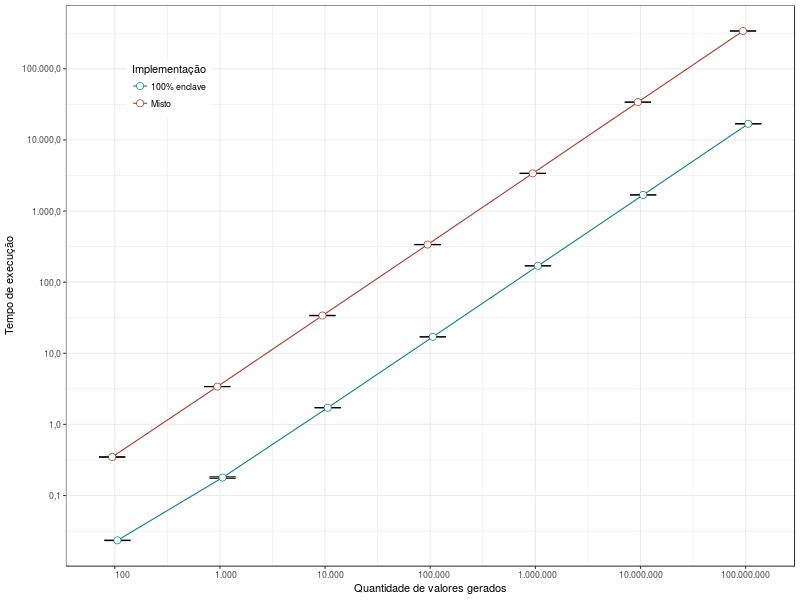
\includegraphics[width=5in]{img/particionamento-aplicacoes-final}
    \caption{Tempos médios para gerar e calcular a soma de $N$ elementos,
    variando $N$ entre, 100 e 100000000, com um intervalo de 95\% de confiança.}
    \label{fig:abordagem_particionamento_aplicacoes}
\end{figure}

\subsection*{Discussão}

A recomendação feita pela Intel, em relação ao particionamento de aplicações, é
de que o enclave contenha apenas o código das funções que lidam diretamente com
dados sensíveis, com o objetivo de manter o TCB o menor possível. Considerando
os resultados obtidos neste experimento, porém, podemos notar que nem sempre
esta divisão será viável, devido à grande sobrecarga gerada no tempo de execução
da aplicação. Esta sobrecarga acontece pelo fato de que, a cada execução de uma
OCall, o processador precisa realizar uma troca de contexto do modo enclave para
o modo normal, e de volta para o modo enclave ao terminar a execução da OCall.
Desta forma, recomendamos que funções da parte insegura que têm muita interação
com funções do enclave da aplicação também sejam implementadas e executadas
dentro do enclave.

% \section{Colocação de aplicações}
% \label{sec:abordagem_colocacao_aplicacoes}

% Na grande maioria das vezes, várias aplicações são executadas simultaneamente em
% um mesmo \textit{host}. Nestas condições, tais aplicações disputam os recursos
% disponíveis na máquina. \fixme{Continua...}

% \subsection*{Experimentos}

% \fixme{Usar o stress}\footnote{\url{http://www.nanoshots.com.br/2016/03/stress-realizando-testes-de-estresse-de.html}}

% \subsection*{Resultados obtidos}

% \subsection*{Discussão}

% \section{Primitivas criptográficas}
% \label{sec:abordagem_primitivas_cripto}

% Como parte da solução SGX, são disponibilizadas diferentes implementações de
% primitivas criptográficas. \fixme{Continua...}

% \subsection*{Experimentos}

% \subsection*{Resultados obtidos}

% \subsection*{Discussão}